\documentclass[spanish,12pt]{article}

\usepackage{enumitem}
\usepackage{tikz}
\usepackage{pgfplots}
\usepackage{amssymb}
\usepackage{booktabs}
\usepackage{enumerate}
\usepackage{multirow}
\usepackage{amsmath}
\usepackage{graphicx}
\usepackage[margin=1in]{geometry}
\usepackage{indentfirst}
\usepackage[spanish]{babel}
\usepackage[utf8]{inputenc}
\usepackage{fancyhdr}
\usepackage{tikz-feynman}
\usepackage{physics}
\usepackage{color}
\renewcommand{\baselinestretch}{1.5}

\newcommand{\dydx}{\frac{dy}{dx}}
\newcommand{\ddx}{\frac{dy}{dx}}
\newcommand{\R}{\mathbb{R}}
\newcommand{\Z}{\mathbb{Z}}
\newcommand{\N}{\mathbb{N}}
\newcommand*\Eval[3]{\left.#1\right\rvert_{#2}^{#3}}
\def\cotan{\qopname\relax o{cotan}}

\setlength{\parskip}{0.4cm}

\pagestyle{fancy}
\fancyhead{}
\fancyfoot{}
\usepackage{titlesec}
\titleformat{\section}
  {\normalfont\Large\bfseries}{\thesection}{1em}{}[{\titlerule[0.8pt]}]
\usepackage{hyperref}
\hypersetup{
    colorlinks=true,
    linkcolor=blue,
    filecolor=magenta,      
    urlcolor=cyan,
    pdftitle={Solucionario P3},
}
\fancyhead[l]{\fontsize{8}{12}\slshape\MakeUppercase{Métodos de prueba}}
\fancyhead[R]{\slshape{J. Pulido}}
\fancyfoot[c]{\thepage}
\pgfplotsset{compat=1.17}
\begin{document}
	\begin{titlepage}
	\begin{center}
	\hspace{0pt}
	\vfill
	Trigonometría – IV
	\medskip
	
	{\Large\textbf{{Clase 1: Introducción a la trigonometría}}}
	
	\medskip
	Julio Pulido
	\thispagestyle{empty}
	\vfill
	\end{center}
	\end{titlepage}
\newpage
\section{Introducción al Espacio Tridimencional}

Para los ejes $x$, $y$ y $z$ perpendiculares entre sí, un punto $P$ se expresa con coordenadas $P(x,y,z)$.

\subsection{Punto Medio}

El punto medio de dos puntos $A$ y $B$ es aquel que se encuentra a la mínima e igual distancia de ambos. Alternativamente se puede definir como aquel punto que bisecta\footnote{Bisectar: dividir un segmento, ángulo, etc... en partes iguales.} el segmento $\overline{AB}$.

Si si tienen dos puntos $A(x_a,y_a,z_a)$ y $B(x_b,y_b,z_b)$, su punto medio ($P$) corresponderá a las coordenadas $P\left(\frac{x_a+x_b}{2},\frac{y_a+y_b}{2},\frac{z_a+z_b}{2}\right)$
\newpage
\subsection{Distancia}
En el plano, la distancia entre dos puntos se calcula como:
$$d=\sqrt{(\Delta x)^2+(\Delta y)^2}\quad\quad \text{donde }\quad\Delta x=x_2-x_1 \wedge \Delta y=y_2-y_1$$
Esto proviene del Teorema de Pitágoras\footnote{para un triángulo rectangulo, la suma de los cuadrados de los catetos es igual al cuadrádo de la hipotenusa.}.

\textbf{Investigación propuesta:} Suponga un cubóide distribuido en el espacio tridimencional con vértices $O(0,0,0)$, $A(x,0,0)$, $B(x,y,0)$, $C(0,y,0)$, $D(0,0,z)$, $E(x,0,z)$, $F(x,y,z)$ y $G(0,y,z)$.

Calcule las siguientes distancias:
\begin{enumerate}[I)]
    \item $\overline{OA}$
    \item $\overline{OB}$
    \item $\overline{OF}$
\end{enumerate}
\newpage
En base a esta investigación se deduce que la distancia en el espacio tridimencional se puede representar como:
$$d=\sqrt{(\Delta x)^2+(\Delta y)^2+(\Delta z)^2}$$\footnote{\#Dato\_Freak: la distancia en el espacio $n$-dimensional se puede representar como $d=\sqrt{\sum\limits_{k=1}^{n}(\Delta a_k)^2}$ donde $a_k$ corresponde al $k$-ésimo eje de las $n$ dimensiones.}
\newpage
\section{Trigonometría}
\subsection{Relaciones trigonométricas en un triángulo rectángulo}

Considerando un triángulo rectángulo, se toma la perspectiva de uno de sus ángulos agudos, nombrando los lados como hipotenusa, opuesto al ángulo y adyacente al ángulo.

\begin{figure}[h]
\centering
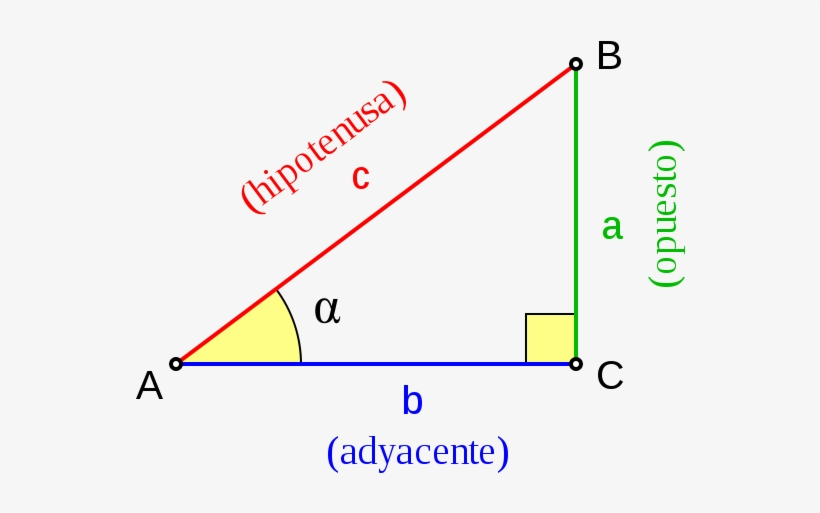
\includegraphics[width=0.4\textwidth]{TR.jpg}
\caption{Triángulo rectángulo}
\end{figure}

Se definen entonces tres relaciones trigonométricas generales en base a los ratios entre los lados:

\begin{align*}
    \sin{\alpha}=\frac{o}{h}\\
    \cos{\alpha}=\frac{a}{h}\\
    \tan{\alpha}=\frac{o}{a}
\end{align*}

Además, se definen los ratios inversos de la siguiente manera:

\begin{align*}
    \cosec{\alpha}&=\frac{1}{\sin{\alpha}}=\frac{h}{o}\\
    \sec{\alpha}&=\frac{1}{\cos{\alpha}}=\frac{h}{a}\\
    \cotan{\alpha}&=\frac{1}{\tan{\alpha}}=\frac{a}{o}
\end{align*}

Es necesario destacar la diferencia de notación entre los ratios inversos y las operatorias inversas a los ratios

\begin{align*}
    \sin^{-1}{\frac{o}{h}}=\arcsin{\frac{o}{h}}=\alpha\\
    \cos^{-1}{\frac{o}{h}}=\arccos{\frac{a}{h}}=\alpha\\
    \tan^{-1}{\frac{o}{h}}=\arctan{\frac{o}{a}}=\alpha
\end{align*}

\newpage
\subsection{Ángulos}

Existen dos formas de uso común para representar ángulos. 

Una de ellas son los \textbf{grados}, donde la amplitud de un ángulo recorre desde $0^{\circ}$ (amplitud nula) hasta $360^{\circ}$ (amplitud total). Cabe mencionar que para ángulos mayores a 360$^{\circ}$ se cumple una identidad cíclica tal que:

$$\theta=\theta+360^{\circ}k\quad\forall\;k\in\Z$$

La otra forma de uso común son los \textbf{radianes}, donde la amplitud de un ángulo recorre desde $0$ (amplitud nula) hasta $2\pi$ (amplitud total). Esta forma se relaciona a las longitudes de arcos proyectados por un ángulo en un círculo unitario\footnote{Círculo de radio 1.}. También aquí se cumple una identidad cíclica tal que:

$$\theta=\theta+2k\pi\quad\forall\;k\in\Z$$

La relación entre un mismo ángulo en radianes ($rad$) y grados ($deg$) se da por la siguiente ecuación:

$$rad=2\pi\frac{deg}{360^{\circ}}$$
\end{document}